% Created 2014-04-08 mar 13:14
\documentclass[xcolor={usenames,svgnames,dvipsnames}]{beamer}
\usepackage[utf8]{inputenc}
\usepackage[T1]{fontenc}
\usepackage{fixltx2e}
\usepackage{graphicx}
\usepackage{longtable}
\usepackage{float}
\usepackage{wrapfig}
\usepackage{rotating}
\usepackage[normalem]{ulem}
\usepackage{amsmath}
\usepackage{textcomp}
\usepackage{marvosym}
\usepackage{wasysym}
\usepackage{amssymb}
\usepackage{hyperref}
\tolerance=1000
\usepackage{color}
\usepackage{listings}
\usepackage{gensymb}
\DeclareMathOperator{\sign}{sign}
\AtBeginSection[]{\begin{frame}[plain]\tableofcontents[currentsection,hideallsubsections]\end{frame}}
\lstset{keywordstyle=\color{blue}, commentstyle=\color{gray!90}, basicstyle=\ttfamily\small, columns=fullflexible, breaklines=true,linewidth=\textwidth, backgroundcolor=\color{gray!23}, basewidth={0.5em,0.4em}, literate={á}{{\'a}}1 {ñ}{{\~n}}1 {é}{{\'e}}1 {ó}{{\'o}}1 {º}{{\textordmasculine}}1}
\usepackage{mathpazo}
\usefonttheme{serif}
\usecolortheme{rose}
\usetheme{Goettingen}
\hypersetup{colorlinks=true, linkcolor=Blue, urlcolor=Blue, breaklinks=true}
\usepackage[citestyle=authoryear,bibstyle=authoryear,doi=true,url=true]{biblatex}
\let\cite\parencite
\addbibresource{/home/oscar/Dropbox/bibliografia/BibUTF8.bib}
\setbeamertemplate{bibliography item}{}
\setbeamercolor{alerted text}{fg=red!50!black} \setbeamerfont{alerted text}{series=\bfseries}
\usetheme{default}
\author{Oscar Perpiñán Lamigueiro (UPM)}
\date{Abril de 2014}
\title{Control de Calidad de Datos \\ Modelos de Radiación Solar}
\hypersetup{
  pdfkeywords={},
  pdfsubject={},
  pdfcreator={Emacs 24.3.1 (Org mode 8.2.1)}}
\begin{document}

\maketitle

\section{Estadística}
\label{sec-1}


\begin{frame}[label=sec-1-1]{Variable aleatoria y proceso estocástico}
\begin{itemize}
\item Una \alert{variable aleatoria} es una función que asigna un único numero
real a cada resultado de un espacio muestral en un experimento.
\item Un \alert{proceso estocástico} es una variable aleatoria que evoluciona a
lo largo del \alert{tiempo} (p.ej. la radiación).
\end{itemize}
\end{frame}

\begin{frame}[label=sec-1-2]{Función de densidad de probabilidad}
La función de densidad de probabilidad, $f(X)$, de una variable
aleatoria \alert{asigna probabilidad} a un suceso:


\[
P(a<X<b)=\int_{a}^{b}f(x)dx
\]


\[
P(X<b)=\int_{-\infty}^{b}f(x)dx\]


\[
P(X>a)=\int_{a}^{\infty}f(x)dx\]
\end{frame}

\begin{frame}[label=sec-1-3]{Función de Densidad de Probabilidad}
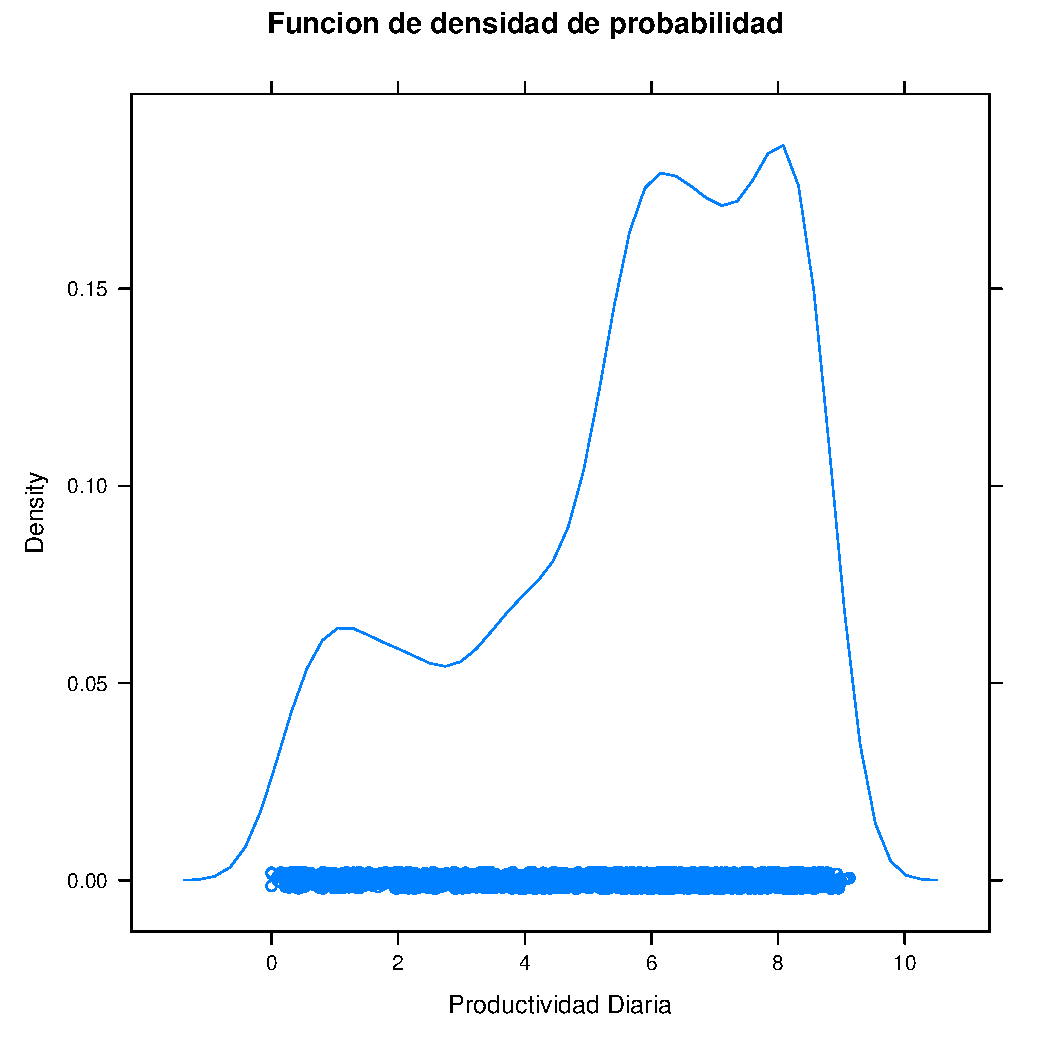
\includegraphics[width=.9\linewidth]{/home/oscar/Copy/Docencia/LibroESF/Figuras/FuncionDensidadProbabilidad.pdf}
\end{frame}
\begin{frame}[label=sec-1-4]{Histograma}
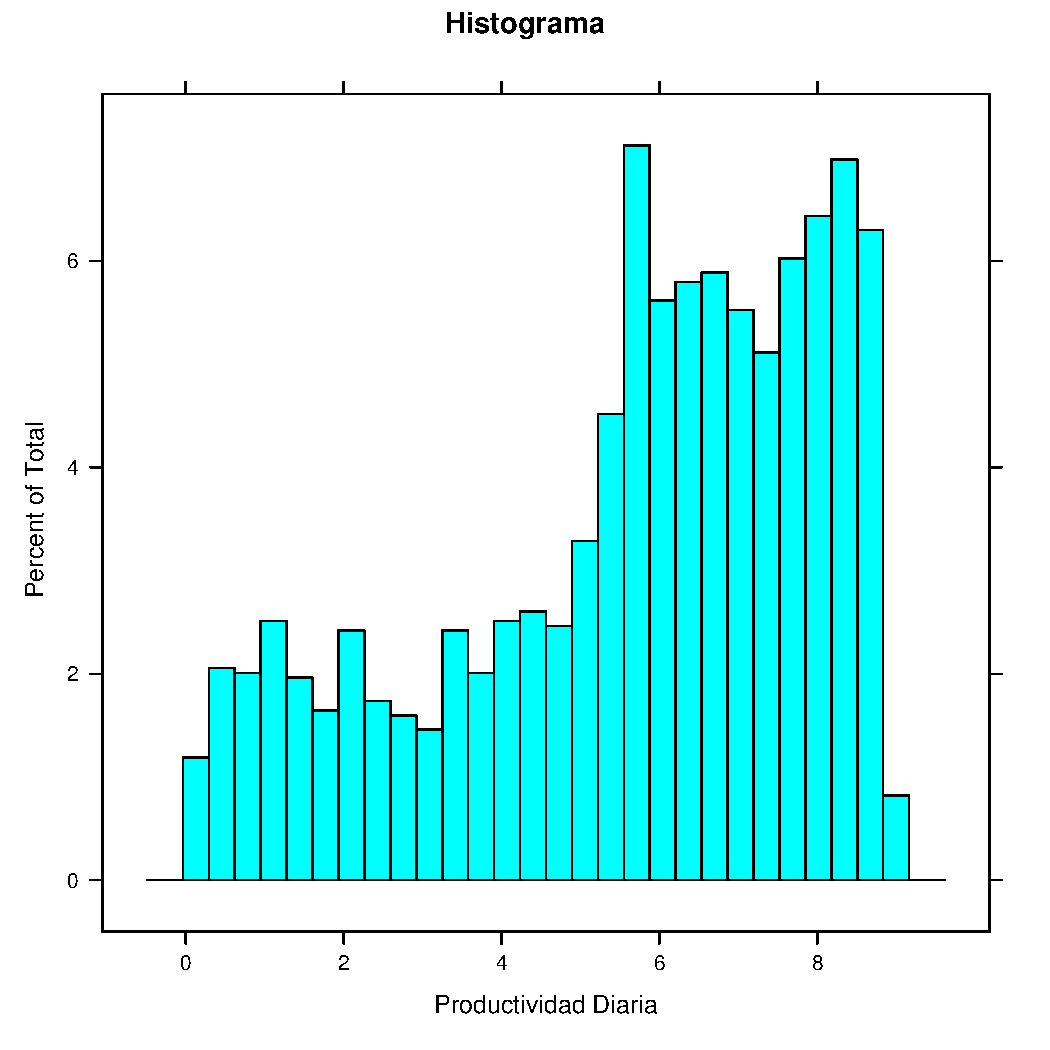
\includegraphics[width=.9\linewidth]{/home/oscar/Copy/Docencia/LibroESF/Figuras/Histograma.pdf}
\end{frame}


\begin{frame}[label=sec-1-5]{Media, varianza y desviación estándar}
\begin{itemize}
\item La \alert{media} de una variable aleatoria es el \alert{centro de masas} de su función densidad de probabilidad:
\end{itemize}

\[
\mu_{X}=\int_{-\infty}^{\infty}x\cdot f(x)dx
\]

\begin{itemize}
\item La \alert{varianza} de una variable aleatoria es la \alert{media del cuadrado de las desviaciones} respecto a la media:
\end{itemize}

\[
\sigma_{X}^{2}=\int_{-\infty}^{\infty}(x-\mu_{X})^{2}\cdot f(x)dx
\]

\begin{itemize}
\item La \alert{desviación estándar} es la raiz cuadrada de la varianza: $\sigma_{X}=\sqrt{\sigma_{X}^2}$
\end{itemize}
\end{frame}


\begin{frame}[label=sec-1-6]{Combinación lineal de variables aleatorias}
\begin{itemize}
\item La \alert{media de la suma} de varias variables aleatorias \alert{independientes} es
la suma de las medias:
\end{itemize}
\[
\mu_{X_{1}+...+X_{n}}=\mu_{X_{1}}+...+\mu_{X_{n}}
\]

\begin{itemize}
\item La \alert{varianza de la \emph{suma o resta}} de varias variables aleatorias
  \alert{independientes} es la \alert{suma} de las varianzas:
\end{itemize}

\[
\sigma_{X_{1}\pm...\pm X_{n}}^{2}=\sigma_{X_{1}}^{2}+...+\sigma_{X_{n}}^{2}
\]
\end{frame}


\begin{frame}[label=sec-1-7]{Media y varianza de la media muestral}
\begin{itemize}
\item Una \alert{muestra de una población} es un conjunto de variables
aleatorias independientes ($X_{1}...X_{n}$).

\item Si se toma una muestra de una población cuya media es $\mu$ y su
varianza es $\sigma^{2}$, entonces la media de la muestra es otra
variable aleatoria (que es una suma de variables aleatorias)
\end{itemize}

\[
\overline{X}=\frac{1}{n}\sum_{n}X_{i}
\]
\end{frame}


\begin{frame}[label=sec-1-8]{Media y varianza de la media muestral}
\begin{itemize}
\item Por tanto, la \alert{media de la media muestral} es la media de población:
\end{itemize}
\[
\overline{X}=\frac{1}{n}\sum_{n}X_{i} = \mu
\]

\begin{itemize}
\item La \alert{varianza de la media muestral} es la suma de las varianzas:
\end{itemize}

\[
\sigma_{\overline{X}}^{2}=\sigma_{\frac{1}{n}X_{1}}^{2}+...+\sigma_{\frac{1}{n}X_{n}}^{2}=\frac{\sigma^2}{N}
\]

Por tanto, una forma de \alert{reducir la incertidumbre} es realizar la
\alert{medida en repetidas ocasiones}.
\end{frame}


\begin{frame}[label=sec-1-9]{Mediana y cuartiles}
\begin{itemize}
\item La \alert{mediana} divide el conjunto de valores de la variable en \alert{dos
mitades} iguales (divide el area encerrada por la función densidad
de probabilidad en dos partes iguales).
\item Los \alert{cuartiles} dividen este area en \alert{cuatro} partes iguales.
\item El area encerrada entre cada par de cuartiles es igual al 25\% del total.
\item La \alert{mediana} es el \alert{segundo cuartil}.
\item La \alert{distancia intercuartil} (definida entre los cuartiles 1 y 3) es
una \alert{medida de la dispersión} de la variable.
\end{itemize}
\end{frame}

\section{Gráficos}
\label{sec-2}


\begin{frame}[label=sec-2-1]{Función de Densidad de Probabilidad}
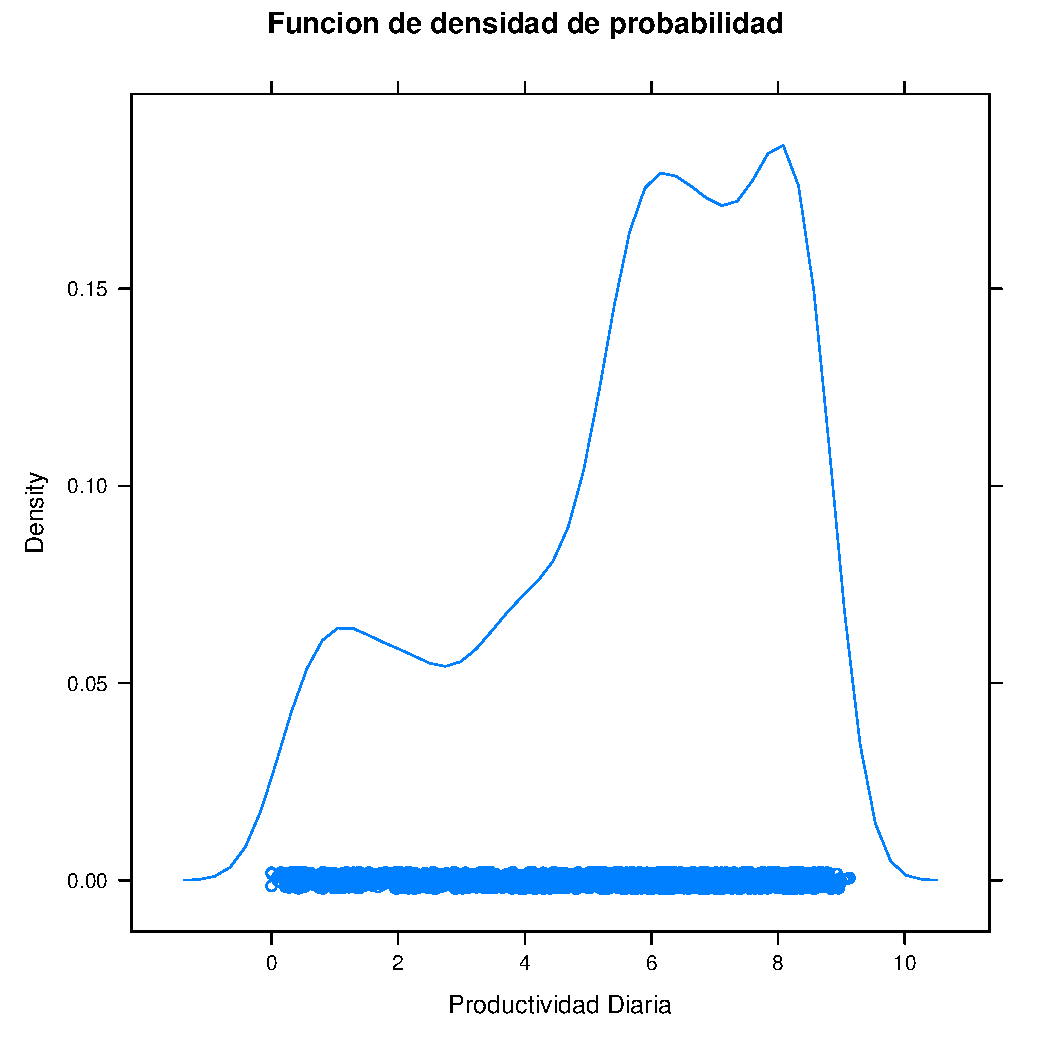
\includegraphics[width=.9\linewidth]{/home/oscar/Copy/Docencia/LibroESF/Figuras/FuncionDensidadProbabilidad.pdf}
\end{frame}
\begin{frame}[label=sec-2-2]{Histograma}
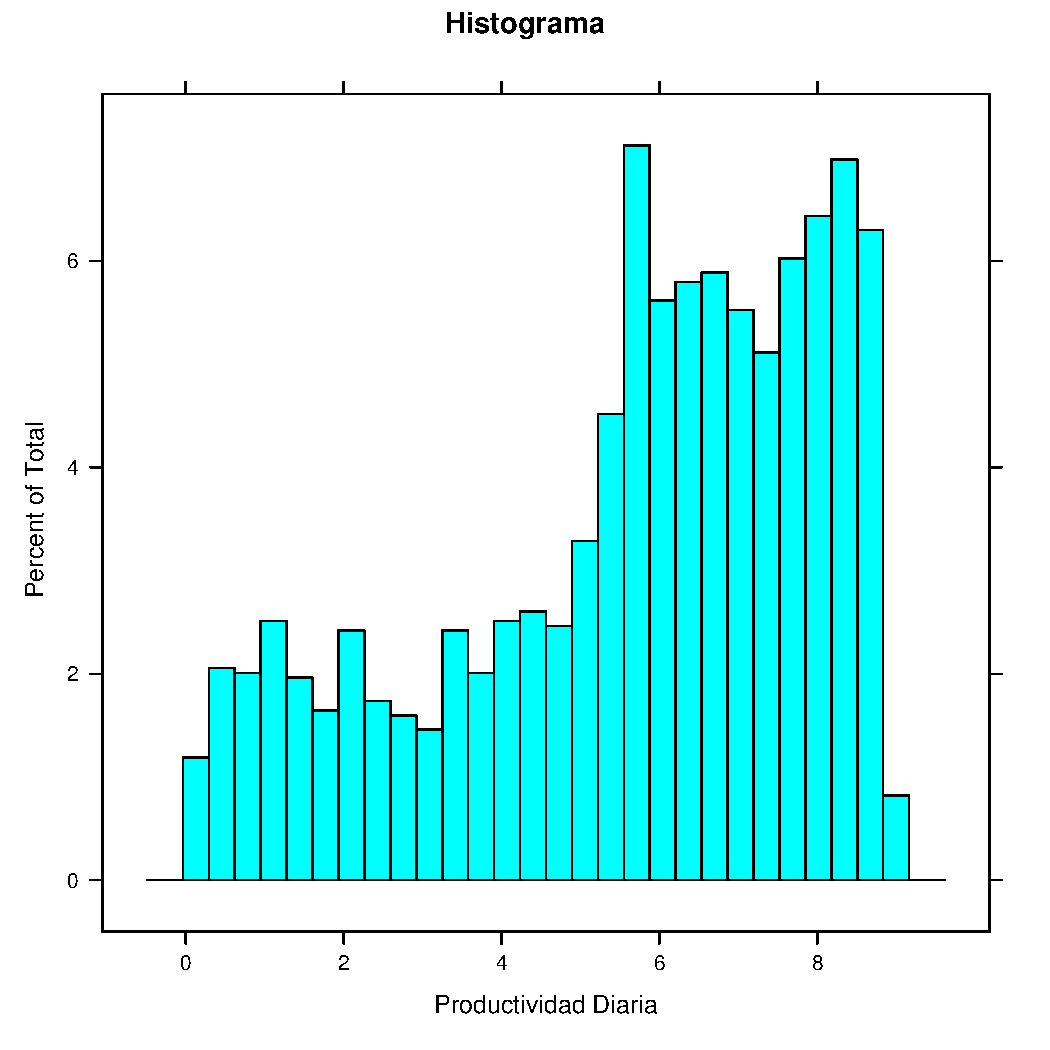
\includegraphics[width=.9\linewidth]{/home/oscar/Copy/Docencia/LibroESF/Figuras/Histograma.pdf}
\end{frame}

\begin{frame}[label=sec-2-3]{Gráficos boxplot}
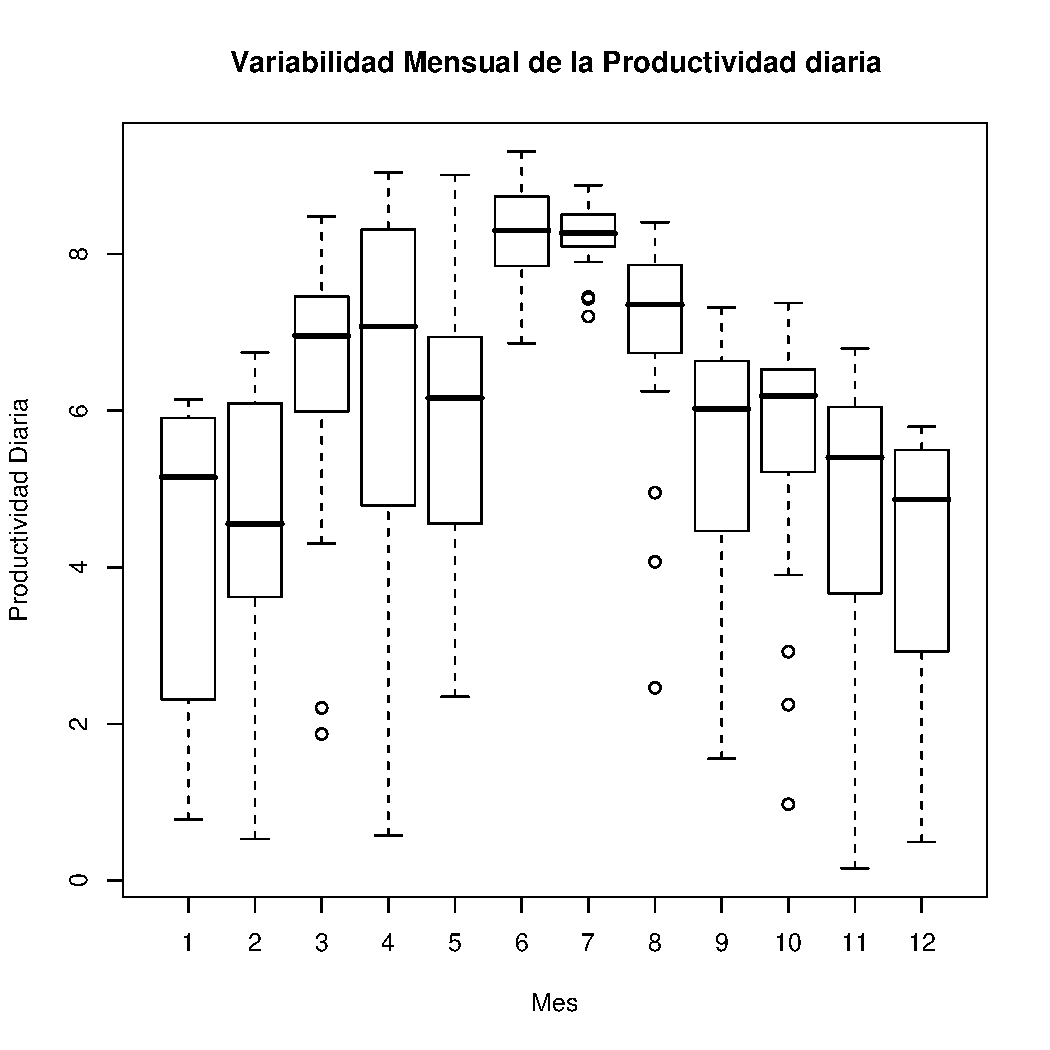
\includegraphics[width=.9\linewidth]{/home/oscar/Copy/Docencia/LibroESF/Figuras/GraficoBoxplot.pdf}
\end{frame}

\begin{frame}[label=sec-2-4]{Gráficos de dispersión}
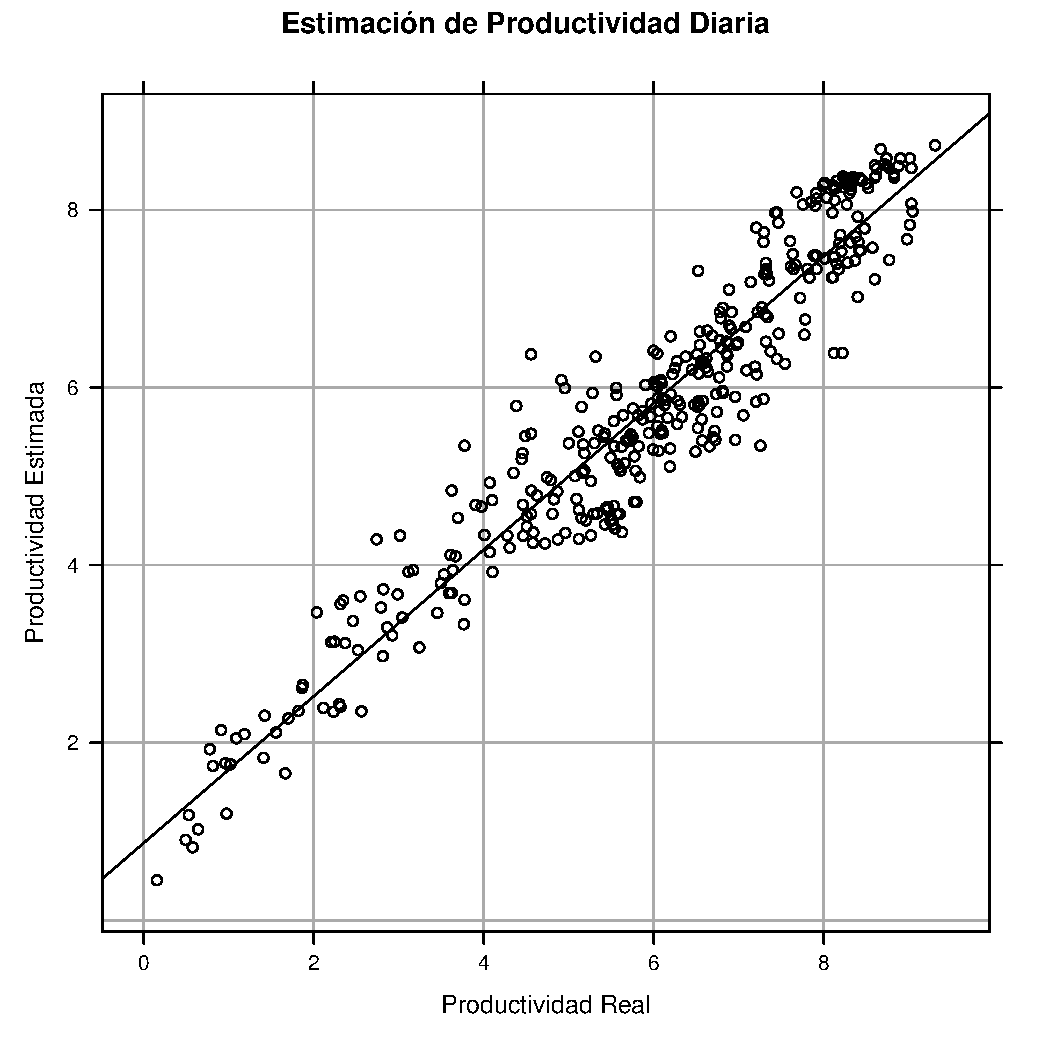
\includegraphics[width=.9\linewidth]{/home/oscar/Copy/Docencia/LibroESF/Figuras/GraficoDispersion.pdf}
\end{frame}

\begin{frame}[label=sec-2-5]{Matrices de gráficos de dispersión}
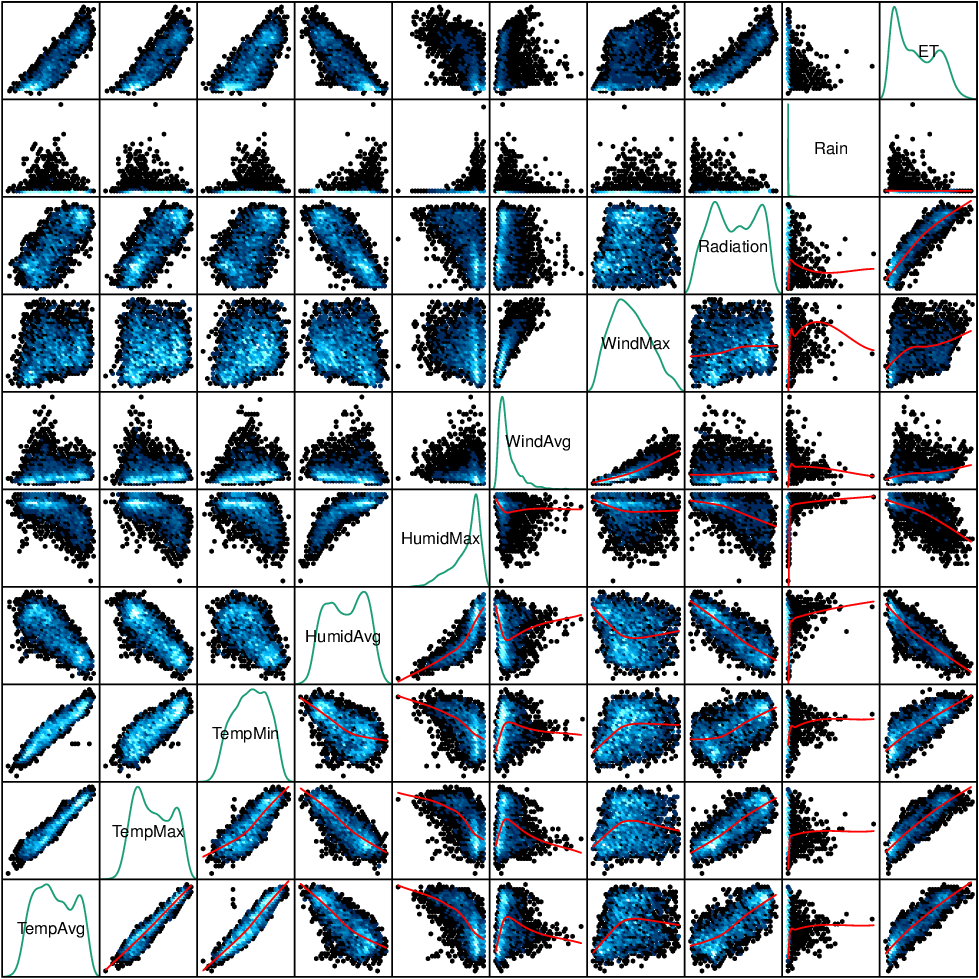
\includegraphics[height=0.9\textheight]{/home/oscar/Copy/Docencia/LibroESF/Figuras/Splom.png}
\end{frame}
\section{Control de Calidad de Medidas}
\label{sec-3}

\begin{frame}[label=sec-3-1]{Introducción}
\begin{block}{Las medidas recogidas por estaciones meteorológicas se deben filtrar para eliminar datos erroneos.}
\begin{itemize}
\item Límites Físicos
\item Tests de persistencia
\item Tests de rampas (irradiancia)
\item Tests de envolvente (medida de varias componentes)
\item Coherencia espacial
\item Coherencia estadística
\end{itemize}
\end{block}
\end{frame}


\begin{frame}[label=sec-3-2]{Límites físicos}
\begin{block}{Irradiación Diaria}
\begin{itemize}
\item La radiación global en el plano horizontal debe ser inferior a la extraterrestre ($K_t \leq 1$)
\end{itemize}
\[
G_d(0) \leq B_od(0)
\]

\begin{itemize}
\item El índice de claridad debe ser superior a 0.03
\end{itemize}
\[
K_t = \frac{G_d(0)}{B_{od}(0)} \geq 0.03
\]

\begin{itemize}
\item La radiación global en el plano horizontal debe ser inferior a la de un modelo de cielo claro
\end{itemize}

\cite{Younes.Claywell.ea2005, Estevez.Gavilan.ea2011, Geiger.Diabate.ea2002}
\end{block}
\end{frame}
\begin{frame}[label=sec-3-3]{Límites físicos}
\begin{block}{Irradiancia (intradiaria)}
\begin{itemize}
\item El índice de claridad debe ser inferior a 1 cuando la altura solar es suficiente:
\end{itemize}
\[
k_t < 1  \text{ si } \gamma_s > 2\degree 
\]
\begin{itemize}
\item Límites inferiores para cielos cubiertos (baja transparencia atmosférica)
\end{itemize}
\[
k_t \geq 10^{-4} \cdot (\gamma_s - 10\degree)  \text{ si } \gamma_s > 10\degree
\]

\[
G \geq 0  \text{ si } \gamma_s \leq 10\degree
\]

\cite{Journee.Bertrand2011}
\end{block}
\end{frame}
\begin{frame}[label=sec-3-4]{Tests de persistencia}
\begin{block}{Variabilidad de irradiancia}
\begin{itemize}
\item La media y la desviación estándar se calculan con todas las muestras de un día completo.
\end{itemize}
\[
\frac{1}{8} \overline{k_t} \leq \sigma_{k_t} \leq 0.35
\]
\end{block}
\end{frame}
\begin{frame}[label=sec-3-5]{Tests de rampas}
\begin{block}{Límites a las variaciones de la irradiancia entre instantes sucesivos}
\[
\left| k_t(t) - k_t(t-1)\right| < 0.75 \text{ si } \gamma_s(t) > 2\degree
\]
\end{block}
\end{frame}

\begin{frame}[label=sec-3-6]{Tests de envolvente}
\begin{itemize}
\item Sólo para estaciones con medida simultánea de global y directa/difusa.
\end{itemize}

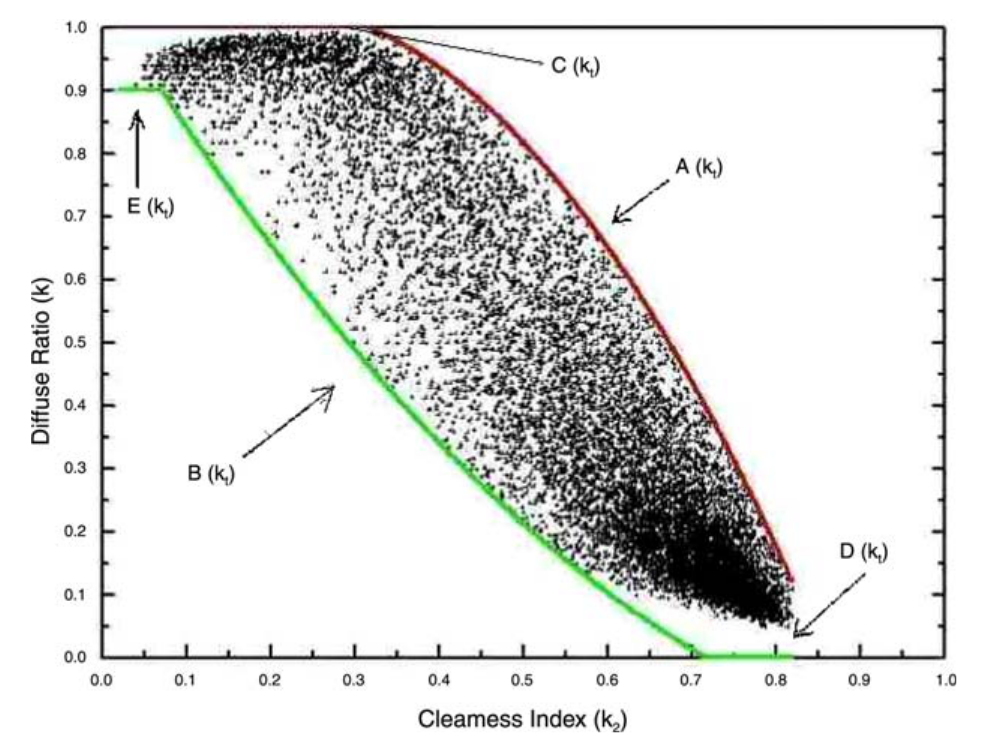
\includegraphics[width=.9\linewidth]{/home/oscar/Copy/Docencia/LibroESF/Figuras/ConsistencyTest.png}

\cite{Younes.Claywell.ea2005}
\end{frame}
\begin{frame}[label=sec-3-7]{Coherencia espacial}
\begin{itemize}
\item Las medidas de una estación se pueden comparar con las recogidas por estaciones cercanas.
\item Esta comprobación debe realizarse con \alert{datos agregados} (diarios) (la variabilidad espacial intradiaria puede ser alta)
\item Esta comprobación debe realizarse con estaciones que tienen \alert{clima y geografía similar}.
\end{itemize}

\cite{Journee.Bertrand2011}
\end{frame}
\begin{frame}[label=sec-3-8]{Coherencia espacial}
\begin{block}{Pasos}
\begin{itemize}
\item Estimamos la irradiación en el lugar, $x_0$, con la interpolación espacial de las estaciones cercanas, $x_i$.
\begin{itemize}
\item Los pesos $w_i$ son una función inversa de la distancia (IDW).
\end{itemize}
\end{itemize}
\[
\widehat{G}_d(x_0) = \frac{\sum_{i=1}^N w_i G_{d}(x_i)}{\sum_{i=1}^N w_i} 
\]
\begin{itemize}
\item Comparamos la irradiación estimada, $\widehat{G}_d(x_0)$, con la medida en la estación, $G_d(x_0)$.
\end{itemize}
\[
\left| \widehat{G}_d(x_0) - G_d(x_0) \right|
\]
\begin{itemize}
\item La diferencia absoluta debe estar por debajo de un límite (p.ej. 50\%)
\end{itemize}
\end{block}
\end{frame}


\begin{frame}[label=sec-3-9]{Coherencia estadística}
\begin{block}{Una medida puede ser etiquetada como \emph{outlier} si es poco probable que pertenezca a la misma distribución que el conjunto.}
\end{block}
\begin{block}{\alert{Método de Chauvenet}}
Una medida es un \emph{outlier} si la probabilidad de obtener su desviación
respecto de la media es inferior al inverso de 2 veces el número de
elementos en el conjunto.

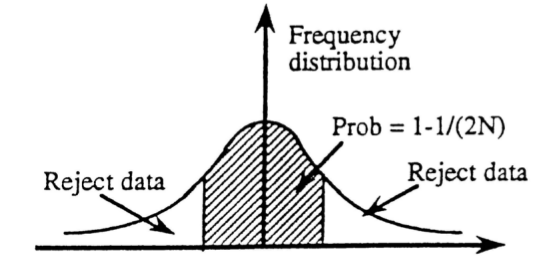
\includegraphics[width=.9\linewidth]{/home/oscar/Copy/Docencia/LibroESF/Figuras/chauvenet.png}
\end{block}
\end{frame}
\begin{frame}[label=sec-3-10]{Método de Chauvenet}
\begin{itemize}
\item Sean $G_d(x_i)$ las medidas de radiación diaria del conjunto formado por N estaciones.
\end{itemize}

\pause

\begin{itemize}
\item Se calcula la media, $\overline{G}_d$, la desviación estándar, $\sigma_{G_d}$.
\end{itemize}

\pause

\begin{itemize}
\item Se calcula la distancia estadística de cada estación al conjunto:
\end{itemize}
\[
d_i = \frac{G_d(x_i) - \overline{G}_d}{\sigma_{G_d}}
\]

\pause

\begin{itemize}
\item En una distribución gaussiana se calcula la distancia estadística
equivalente a la probabilidad límite, $1/2N$, teniendo en cuenta
las dos colas.
\begin{itemize}
\item Por ejemplo, para un conjunto de 10 estaciones cada cola es
      $1/40 = 0.025$, el límite es $\left| d_{max} \right| = 1.96$.
\end{itemize}
\end{itemize}
\pause

\begin{itemize}
\item Aquellas observaciones que superan la distancia son marcadas como outliers.
\end{itemize}

\cite{Perpinan2009}
\end{frame}
\begin{frame}[label=sec-3-11]{Método de Chauvenet}
\[
d_i = \frac{G_d(x_i) - \overline{G}_d}{\sigma_{G_d}}
\]

\[
\left| d_i \right| > \left| d_{max} \right|
\]

\begin{center}
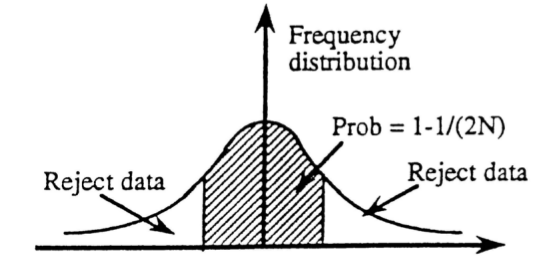
\includegraphics[width=.9\linewidth]{/home/oscar/Copy/Docencia/LibroESF/Figuras/chauvenet.png}
\end{center}

\begin{block}{Método de Pierce: más robusto y flexible \cite{Ross2003}}
\end{block}
\end{frame}
\section{Control de Calidad de Modelos}
\label{sec-4}

\begin{frame}[label=sec-4-1]{Desviación entre modelo y observación}
\begin{itemize}
\item Sea $O$ el conjunto de observaciones (medidas) de una variable aleatoria.
\end{itemize}

\[
\mathbf{O} = \left\{ o_1 \dots o_n \right\}
\]
\begin{itemize}
\item Sea $M$ el conjunto de resultados de un modelo que aproxima el comportamiento de la variable medida.
\end{itemize}

\[
\mathbf{M} = \left\{ m_1 \dots m_n  \right\}
\]

\begin{itemize}
\item La desviación entre modelo y observación es:
\end{itemize}

\[
\mathbf{D} = \mathbf{O} - \mathbf{M} =  \left\{ (o_1 - m_1) \dots (o_n - m_n)  \right\} = \left\{ d_1 \dots d_n  \right\}
\]
\end{frame}
\begin{frame}[label=sec-4-2]{Estimadores frecuentes: MBD y RMSD}
\begin{itemize}
\item Mean Bias Difference (MBD), diferencia media (indica si el modelo sobreestima o subestima):
\end{itemize}
\[
MBE = \overline{\mathbf{D}} = \overline{\mathbf{O}} - \overline{\mathbf{M}} = \frac{1}{n} \sum_{i=1}^n (o_i - m_i)
\]
\pause
\begin{itemize}
\item Root Mean Square Error (RMSD), diferencia cuadrático media:
\end{itemize}
\[
RMSD = \left(\frac{1}{n} \sum_{i=1}^n d_i^2 \right)^{1/2} =  \left( \frac{1}{n} \sum_{i=1}^n (o_i - m_i)^2  \right)^{1/2}
\]
\end{frame}
\begin{frame}[label=sec-4-3]{Estimadores frecuentes: MBE y RMSD}
\begin{itemize}
\item Varianza de la diferencia (unbiased RMSD):
\end{itemize}
\[
\sigma^2_{\mathbf{D}} = \frac{1}{n} \sum_{i=1}^n (d_i - \overline{\mathbf{D}})^2
\]
\pause

\begin{itemize}
\item El RMSD agrega información del promedio y la varianza de la
diferencia:
\end{itemize}
\[
RMSD^2= \sigma^2_{\mathbf{D}} + \overline{\mathbf{D}}^2
\]
\end{frame}
\begin{frame}[label=sec-4-4]{Otros estimadores: MAD}
\begin{itemize}
\item Mean Absolute Deviation (MAD):
\end{itemize}

\[
MAD = \frac{1}{n} \sum_{i=1}^n \left|d_i\right| =  \frac{1}{n} \sum_{i=1}^n \left|o_i - m_i\right|
\]
\begin{itemize}
\item El RMSD no es robusto (un error puntual puede distorsionar el estimador) y depende del número de muestras:
\end{itemize}
\[
MAD \leq RMSD \leq n^{1/2} MAD
\]

\cite{Willmott.Matsuura.ea2009, Willmott.Matsuura2005a}
\end{frame}
\begin{frame}[label=sec-4-5]{Otros estimadores: t y d}
\begin{itemize}
\item t de Student (valores pequeños indican buen comportamiento del modelo)
\begin{itemize}
\item Permite añadir intervalos de confianza a las diferencias entre
modelo y observación
\end{itemize}
\end{itemize}

\[
t = \left ( \frac{(n-1) MBD^2}{RMSD^2 - MBD^2} \right)^{1/2}
\]

\nocite{Stone1993}

\pause 

\begin{itemize}
\item $d_1$: Índice de concordancia de Willmott.
\begin{itemize}
\item Limitado entre 0 (ausencia de concordancia) y 1 (concordancia total).
\item Robusto frente a \emph{outliers}.
\end{itemize}
\end{itemize}
\[
d_1 = 1 - \frac{\sum_{i=1}^n \left| m_i - o_i \right|}{\sum_{i=1}^n \left(
  \left| m_i - \overline{\mathbf{O}}\right| + \left| o_i -
    \overline{\mathbf{O}} \right| \right)}
\]

\cite{Willmott.Robeson.ea2012}
\end{frame}
\begin{frame}[label=sec-4-6]{Correlación}
El coeficiente de correlación entre dos conjuntos de datos es una
medida numérica de la relación \alert{lineal} entre los dos conjuntos (si la
relación no es lineal, este coeficiente no sirve):

\[
r = \frac{1}{n-1} \cdot \sum_{i=1}^{n} \left( \frac{o_{i}-\overline{\mathbf{O}}}{\sigma_{\mathbf{O}}}\right) \cdot \left(\frac{m_{i}-\overline{\mathbf{M}}}{\sigma_{\mathbf{M}}}\right)
\]
\end{frame}
\begin{frame}[label=sec-4-7]{Diagramas de Taylor}
\begin{itemize}
\item Desarrollando $\sigma^2_{\mathbf{D}}$ y teniendo en cuenta la definición de $r$:
\end{itemize}

  \[
  \sigma^2_{\mathbf{D}} = \sigma^2_{\mathbf{O}}  + \sigma^2_{\mathbf{M}}
- 2 \cdot \sigma_{\mathbf{O}} \cdot \sigma_{\mathbf{M}} \cdot r
  \]
\begin{itemize}
\item Esta relación es semejante a la ley de los cosenos ($c$, $a$, $b$ son lados de un triángulo y $\phi$ es el ángulo opuesto al lado $c$):
\end{itemize}

\[
c^2 = a^2 + b^2 - 2 \cdot a \cdot b \cos\phi
\]
\cite{Taylor2000}
\end{frame}
\begin{frame}[label=sec-4-8]{Diagramas de Taylor}
\[
\sigma^2_{\mathbf{D}} = \sigma^2_{\mathbf{O}}  + \sigma^2_{\mathbf{M}}
- 2 \cdot \sigma_{\mathbf{O}} \cdot \sigma_{\mathbf{M}} \cdot r 
\]

\begin{center}
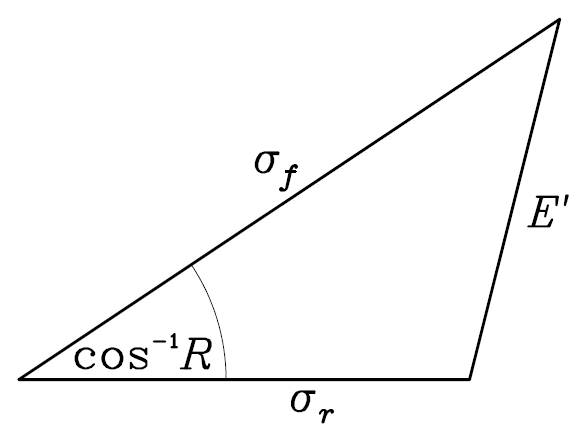
\includegraphics[width=.9\linewidth]{/home/oscar/Copy/Docencia/LibroESF/Figuras/cosenosDiagramaTaylor.png}
\end{center}
\end{frame}
\begin{frame}[label=sec-4-9]{Diagramas de Taylor}
\begin{itemize}
\item $\sigma^2_{\mathbf{D}}$: Distancia al origen
\item $\sigma^2_{\mathbf{O}}$: Eje horizontal
\item $\sigma^2_{\mathbf{M}}$: Eje vertical
\item $r$: acimut
\end{itemize}
\begin{center}
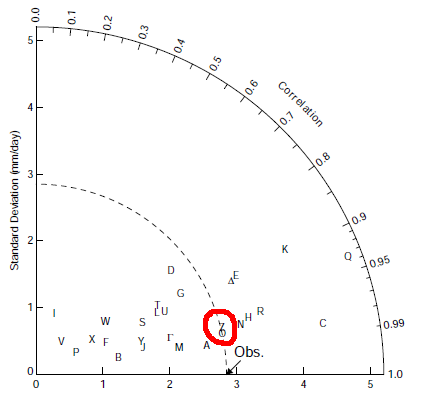
\includegraphics[height=0.6\textheight]{/home/oscar/Copy/Docencia/LibroESF/Figuras/TaylorDiagrama.png}
\end{center}
\end{frame}

\begin{frame}[label=sec-4-10]{Target Diagram}
\begin{itemize}
\item Emplea la relación entre $RMSD$, $\sigma^2_{\mathbf{D}}$, y $\overline{\mathbf{D}}$, normalizadas con $\sigma_{\mathbf{O}}$:
\end{itemize}
\[
RMSD' = RMSD / \sigma_{\mathbf{O}}
\]

\[
  \sigma'_{\mathbf{D}} = \sigma_{\mathbf{D}} / \sigma_{\mathbf{O}} 
\]

\[
\overline{\mathbf{D}}' = \overline{\mathbf{D}} / \sigma_{\mathbf{O}}
\]

\[
RMSD'^2= \sigma'^2_{\mathbf{D}} + \overline{\mathbf{D}}'^2
\]

\begin{itemize}
\item Incorporan el signo de la diferencia entre desviaciones estándar de modelo y observación:
\end{itemize}

\[
sign_{\sigma} =  \sign(\sigma_{\mathbf{M}} - \sigma_{\mathbf{O}} )
\]

\cite{Jolliff.Kindle.ea2009}
\end{frame}
\begin{frame}[label=sec-4-11]{Target Diagram}
\begin{itemize}
\item $\sigma'_{\mathbf{D}}$ (con signo): Eje horizontal
\item $\overline{\mathbf{D}}'$: Eje vertical
\item $RMSD'^2$: Distancia al origen
\end{itemize}

\begin{center}
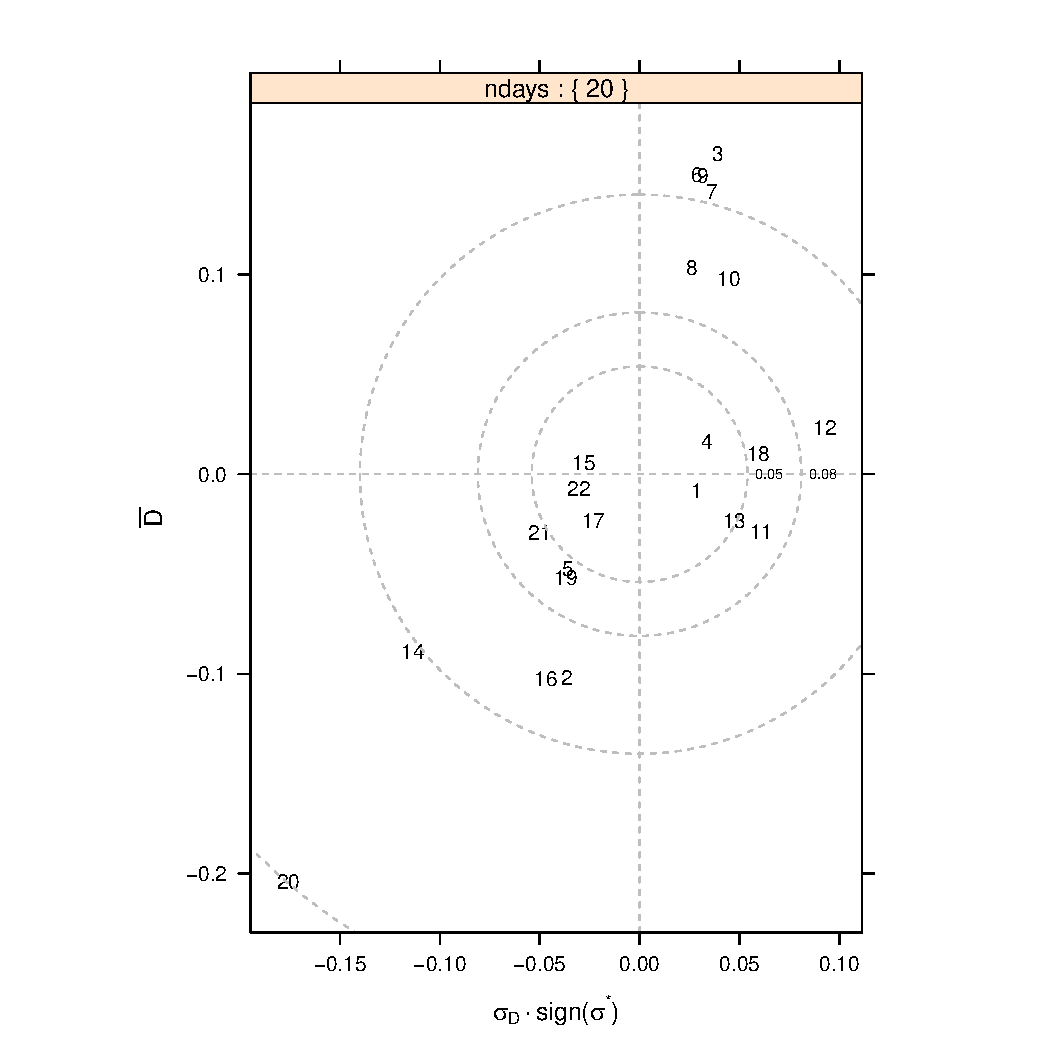
\includegraphics[height=0.7\textheight]{/home/oscar/Copy/Docencia/LibroESF/Figuras/TargetDiagram.pdf}
\end{center}
\end{frame}

\section{Bibliografía}
\label{sec-5}

\begin{frame}[allowframebreaks,label=]{Bibliografía}
\printbibliography
\end{frame}
% Emacs 24.3.1 (Org mode 8.2.1)
\end{document}